\documentclass{article}
\usepackage[UTF8]{ctex}
\usepackage{amsmath,mathtools}
\usepackage{color}
\usepackage{float}
\newcommand{\point}[1]{$\color{blue}{\text{#1}}$}
\title{普物复习}
\author{191220090 沈天杰}
\begin{document}
    \maketitle
    {\centering\tableofcontents}
    \section{静止电荷的电场}
    \noindent基本物理量: 电荷\quad电场强度\quad电势\footnote{电势梯度与场强}\\
    基本定律:电荷守恒定律,库仑定律,场强叠加原理,高斯定律,安培环路定理
    \subsection{电场、电荷\quad库仑定律}
    \[
        \vec{F_{12}}=\frac{1}{4\pi\epsilon_0}\frac{q_1q_2}{r_{12}^2}(\frac{\vec{r_{12}}}{r_{12}})    
    \]
    其中$\frac{1}{4\pi\epsilon_0}\approx 8.988\times 10^9 N\cdot m^2\cdot C^{-2}$\\
    \point{考题}:库仑定律和力的叠加原理
    \subsection{电场\quad电场强度}
    \noindent电场强度是随位置而变的矢量场
    \[
      \vec{E}=\frac{\vec{F}}{q_0}=\frac{Q}{4\pi\epsilon_0r^2} \hat{r} \quad \textbf{点电荷的场强} 
    \]
    场强叠加原理 离散与连续。\\\\
    \point{考题1}:两电荷连线的中垂面上任意一点P的电场强度\\
    电偶极子(或称电偶极矩):$\vec{p}=q\vec{l}$\\
    电偶极子在其延长线上远场点电场强度$E=\frac{p_e}{2\pi\epsilon_0r^3}$
    注意\;1)\;l很小(相对于r) 2)\;方向从负电荷指向正电荷。\\
    点P的电场强度方向与电偶极子相反。电偶极子的电场强度是立方衰减的。\\
    \point{考题2}:无限长均匀带电细棒中垂面上的场强分布\\
    \[
        E_y=\frac{1}{4\pi\epsilon_0}\frac{2\lambda}{a}
    \]
    其中a为待测点到细棒距离。\\
    \point{考题3}:电荷q均匀地分布在半径为R的圆环上,求圆环中心轴线上任一点p的场强。P点离环心的距离为x。\par
    当$x\to \infty$电场强度等同于点电荷\\
    \point{考题4}:均匀带电圆盘在其轴线上产生的电场强度,圆盘半径为R,面密度为$\sigma$:\\
    \[
    E_x=\frac{\sigma}{2\epsilon_0}(1-\frac{1}{\sqrt{1+R^2/x^2}})    
    \]
    1)R$\ll$x \; 点电荷 \\
    2)R$\gg$x \; $E_x=\frac{\sigma}{2\epsilon_0}$ \; 相当于无限大板。匀强电场,和距离无关。\\
    \point{考题5}\textbf{无限大面和无限长线上电荷的综合运用(重点)}
    \begin{figure}[H]
        \centering
        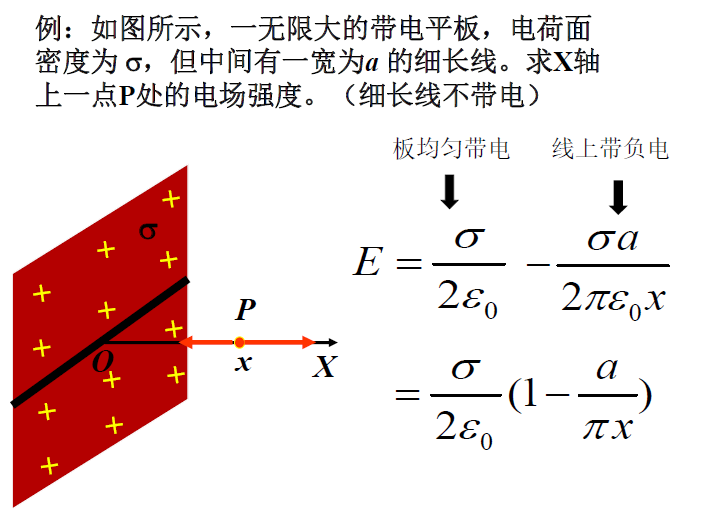
\includegraphics[width=.95\textwidth]{figure/inf.png}
    \end{figure}
    \subsection{电场线}
    \section{恒定电流及其磁场}
    \section{电磁感应、麦克斯韦方程组}
\end{document}